\section{Grafi di test}
Dopo l'implementazione degli algoritmi descritta nel capitolo 4, è stato fatto un test con alcuni grafi arbitrariamente costruiti. Come prima cosa, vengono generati manualmente 4 grafi che rappresentano alcuni degli schemi di catene che potrebbero verificarsi all'interno del tx-graph.

Il primo schema rappresenta il classico cammino dritto, e si può notare in figura \ref{fig:straightgraph}. All'esecuzione dell'algoritmo, viene stampato il path = [0,1,2,3,...,9].
\begin{figure}[htbp]
	\centering
	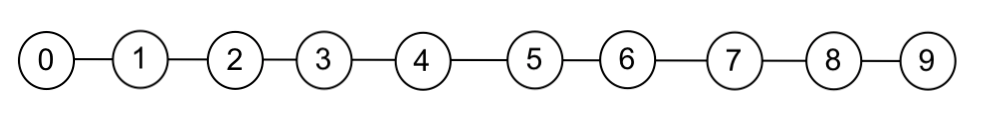
\includegraphics[width = \linewidth]{figure/straightgraph}
	\caption{\textit{Un cammino}\label{fig:straightgraph}}
\end{figure}
Nella figura \ref{fig:ygraph} si può notare un grafo a forma di Y, ovvero due cammini che convergono sullo stesso nodo. Potrebbe essere un classico esempio di una situazione di "merge".
\begin{figure}[htbp]
	\centering
	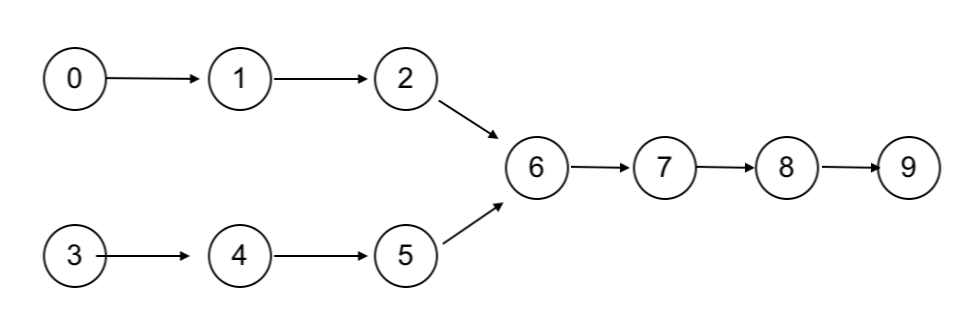
\includegraphics[width = \linewidth]{figure/ygraph}
	\caption{\textit{Un Y grafo}\label{fig:ygraph}}
\end{figure}
Nella fase di test su questo tipo di grafo, tra il nodo 2 e il nodo 5, il nodo 2 ha varianza minore, e il path restituito dall'algoritmo corrisponde proprio a [0,1,2,6,7,8,9].

Nella figura \ref{fig:xgraph} si ha un nuovo schema di grafo a forma di X. Se si esegue l'algoritmo anche su questo, a parità di varianza dei cammini, si otterrà come risultato il path [0,1,2,3,4,5], che è il più lungo.
\begin{figure}[htbp]
	\centering
	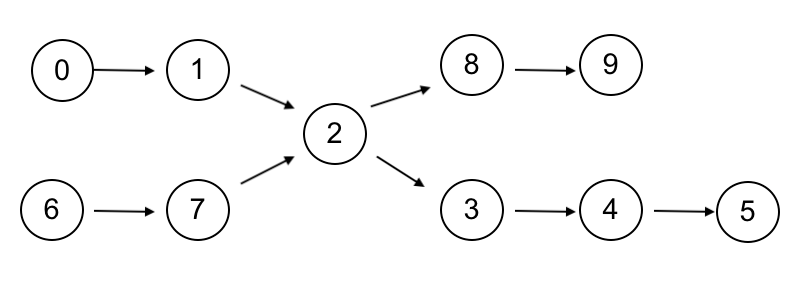
\includegraphics[width = 0.8\linewidth]{figure/xgraph}
	\caption{\textit{Un X grafo}\label{fig:xgraph}}
\end{figure}

Per quanto l'algoritmo del calcolo del cammino più lungo a varianza minima si corretto, a parità di cammini di eguale lunghezza ed egual varianza, stampa solamente il primo di essi, tralasciando gli altri cammini equivalenti.

\section{MatPlotLib per i grafici}
Dopo l'esecuzione dell'algoritmo, quindi, ogni nodo viene etichettato con attributi di frequenza(sia istantanea che media) e varianza. La frequenza istantanea non è molto rilevante per quanto riguarda lo studio sul tx-graph. 

Perciò si è deciso di graficare la distribuzione di tali valori su dei grafici con istogrammi, fatti con una libreria di python chiamata \textbf{MathPlotLib}. I grafici ottenuti rappresentano, sull'asse x la distribuzione dei singoli valori di frequenza(o varianza) dei nodi, e sull'asse y quanti sono quei nodi che hanno tale valore di frequenza(o varianza).

\section{Statistiche \& Grafici}
Inizialmente si è voluto graficare il primo dataset D1(417113, 417256), perchè è quello che più semplicemente si presta a generare un grafico attendibile. Nella figura \ref{fig:histg1} si può notare l'istogramma del primo dataset.
\begin{figure}[htbp]
	\centering
	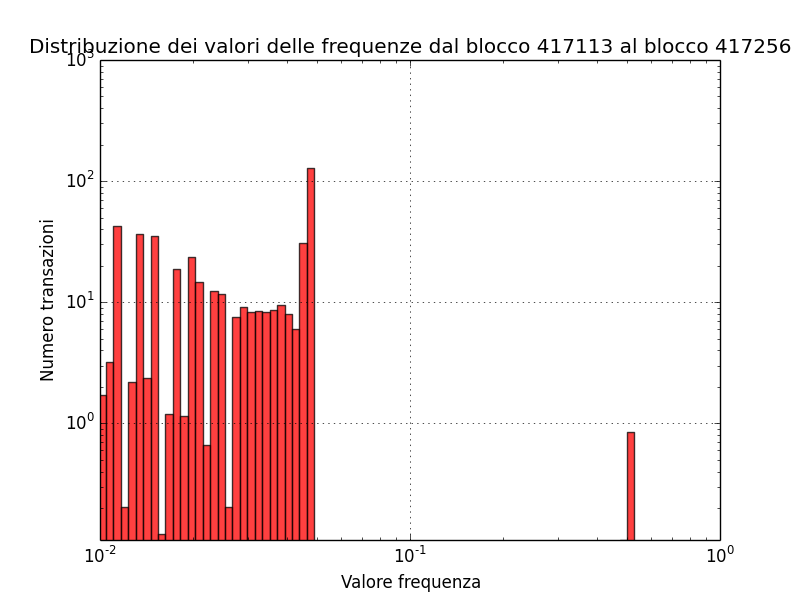
\includegraphics[width = 0.8\linewidth]{figure/histg1}
	\caption{\textit{G1(417113, 417256)}\label{fig:histg1}}
\end{figure}
\newpage
\subsection{Al variare del Dataset}
Prendendo successivamente in considerazione il dataset D2(413000, 414000), e di conseguenza il grafo generato da tale dataset, si è preferito creare dei grafici al variare della dimensione del dataset, per vedere quali erano i valori che si sarebbero aggiunti alla distribuzione.

\begin{figure}[htbp]
	\centering
		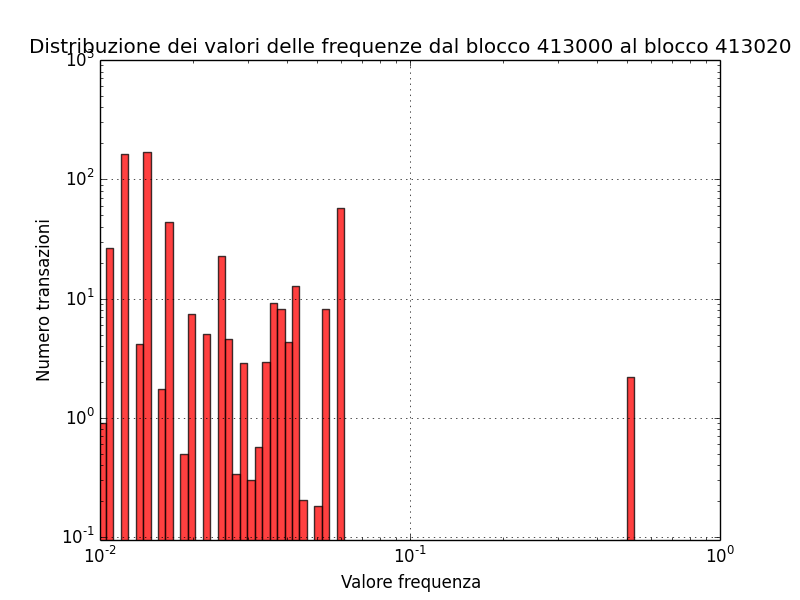
\includegraphics[width=0.7\textwidth]{figure/hist20b}
		\caption{\textit{20 blocchi}\label{fig:hist20b}}
\end{figure}
	
\begin{figure}[htbp]
	\centering
		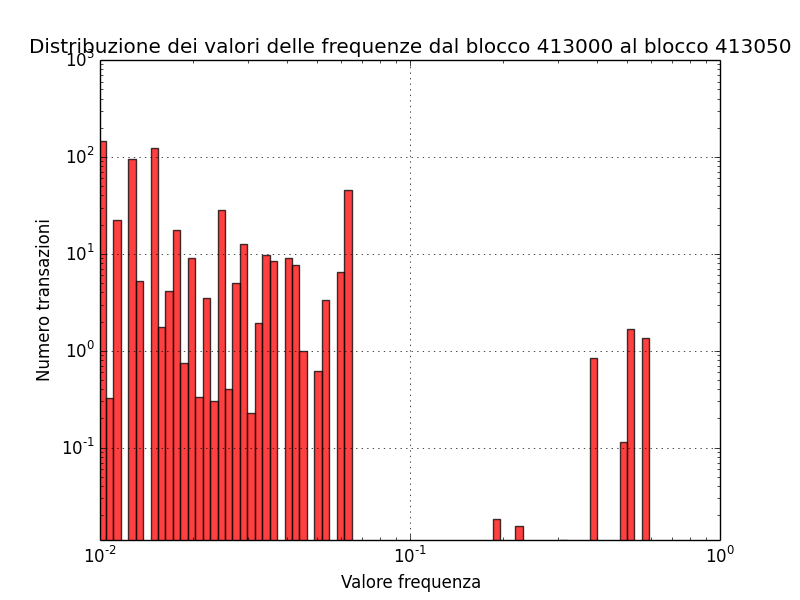
\includegraphics[width=0.7\textwidth]{figure/hist50b}
		\caption{\textit{50 blocchi}\label{fig:hist50b}}
\end{figure}

\begin{figure}[htbp]
	\centering
		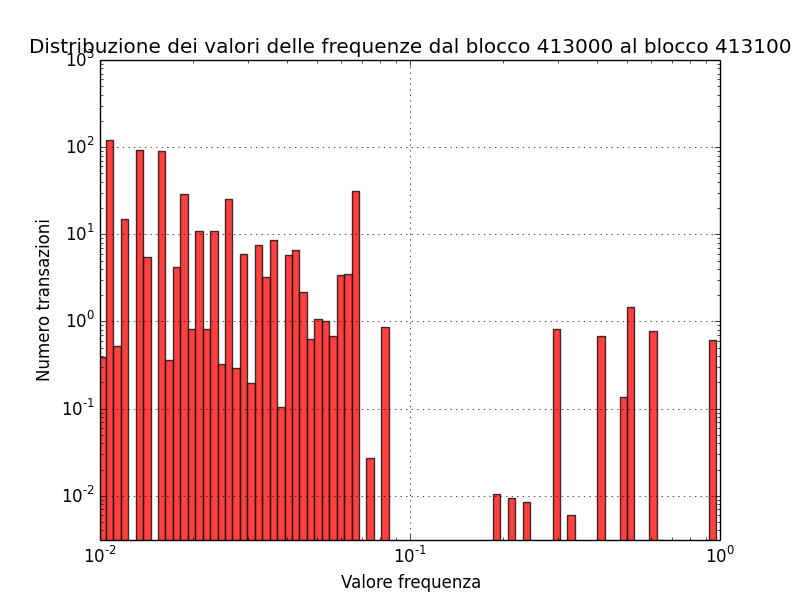
\includegraphics[width=0.7\textwidth]{figure/hist100b}
		\caption{\textit{100 blocchi}\label{fig:hist100b}}
\end{figure}
	
\begin{figure}[htbp]
	\centering
	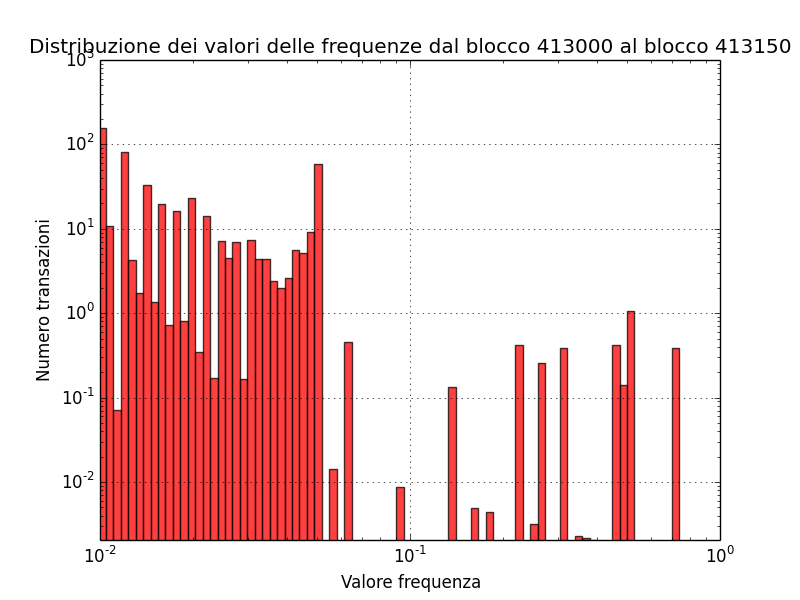
\includegraphics[width=0.7\textwidth]{figure/hist150b}
	\caption{\textit{150 blocchi}\label{fig:hist150b}}
\end{figure}

\begin{figure}[htbp]
	\centering
	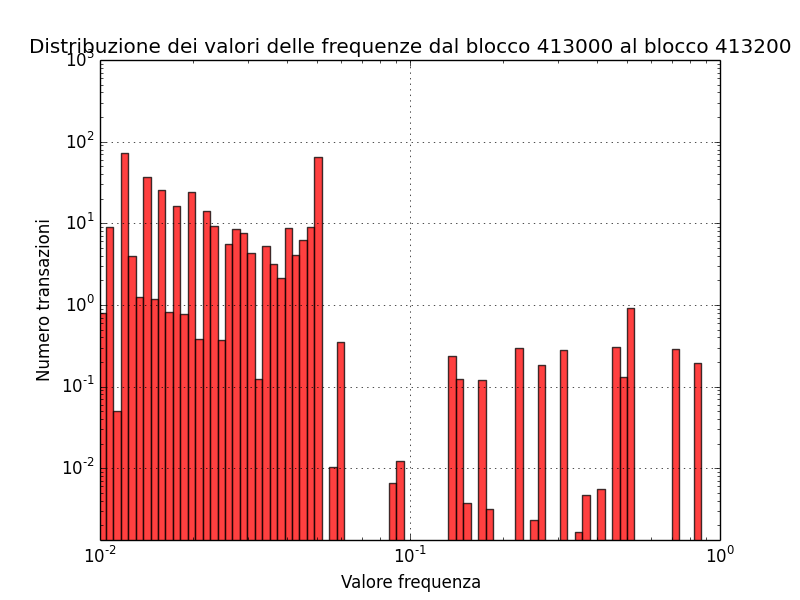
\includegraphics[width=0.7\textwidth]{figure/hist200b}
	\caption{\textit{200 blocchi}\label{fig:hist200b}}
\end{figure}

\begin{figure}[htbp]
	\centering
	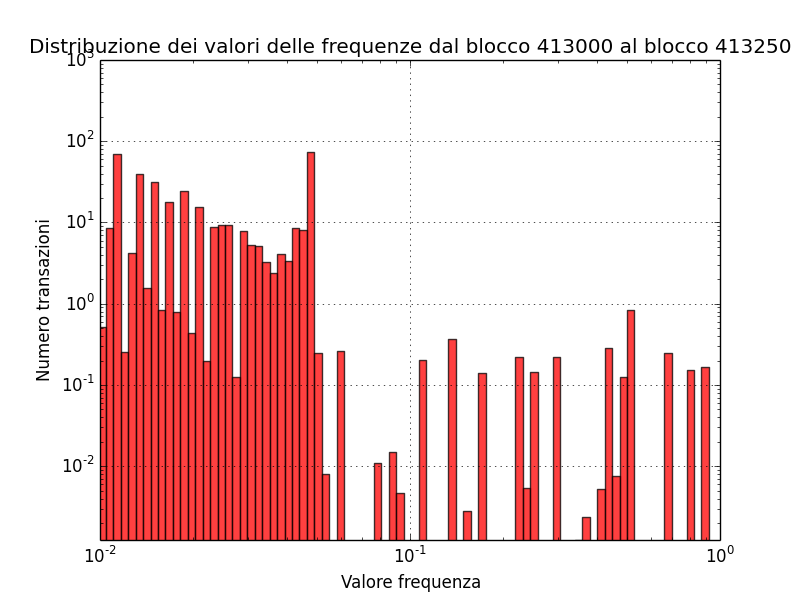
\includegraphics[width=0.7\textwidth]{figure/hist250b}
	\caption{\textit{250 blocchi}\label{fig:hist250b}}
\end{figure}

\begin{figure}[htbp]
	\centering
	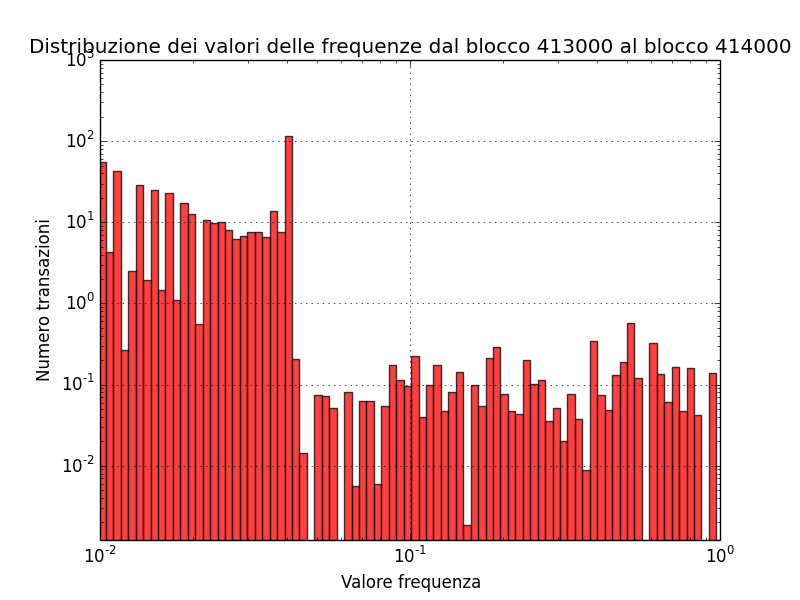
\includegraphics[width=\textwidth]{figure/hist1000b}
	\caption{\textit{1000 blocchi}\label{fig:hist1000b}}
\end{figure}